\chapter{Binary Search Trees (BSTs)}
\label{ch:bst}

%% UPDATE LOG (Umut)
%% Updates from 2014 to 2015 (body-2014.tex)
%% (balancing) scheme --> data structure
%% (I worry that ``scheme'' can piss people off.)
%%
%% skip trees --> skip lists.

Searching is one of the most important operations in computer science.
Of the many search data structures that have been designed and are used
in practice, search trees, more specifically balanced binary search
trees, occupy a coveted place because of their broad applicability to
solving many different sorts of algorithmic problems.  For example, in
this \bc, we rely on binary search trees to implement set and table
abstract data types (\chref{sets-tables}), which are then used in the
implementation of many algorithms, including for example graph
algorithms.


\begin{question}
Can't we use sequences for searching? 
\end{question}
If we are interested in searching a static or unchanging collection of
elements, then we can easily use sequences.  For example, if we use
array-based implementation and cost specification, we can implement an
efficient search function by representing our collection as a sorted
sequence and by using binary search, which would require indexing into
the sequence logarithmically many number of times.
%
If, however, we want to support a dynamic collection, where for
example, we insert new elements and delete existing elements, we would
need linear work.
% 
Binary search trees (BSTs) make it possible to compute with dynamic
collection by using insertions, deletions, as well as searches all in
logarithmic number of tree operations.

In \bcs on sequential algorithms, presentation of binary search trees
focus on functions for inserting elements, for deleting elements, and
for searching.
%
While these functions are important, they are not sufficient for
parallelism, because they perform singleton updates. 
% 
In this \bc, we also consider aggregate update operations, 
such as union and intersection, which can be used to insert and delete (respectively) many elements at once.

%%%% Repetition.
%% deleting keys in/from a tree, we focus on two functions called split
%% and join.  Split chops a tree into two pieces, and join glues pieces
%% back together.  Split and join can be used to efficiently implement
%% insertion and deletion, but also to implement parallel algorithms for
%% functions such as union and intersection.


\section{Preliminaries}

\paragraph{Definitions and Terminology.} 
We start with some basic definitions and terminology involving rooted
and binary search trees.  An example of a rooted tree along with the
associated terminology is given in Example~\ref{ex:rootedtree}, and an
example of a binary search tree is given in Example~\ref{ex:bst}.
%

Briefly, summarizing, a rooted tree is a tree with a distinguished
root node that can be used to access all other nodes
(\defref{rootedtree}).
%
A binary tree full binary tree is a rooted tree, where each node is
either a leaf or an internal node with a left and a right child (\defref{binarytree}). 
%
A binary search tree is a binary tree, where each internal node $u$
has a unique key~$k$ such that each node in its left subtree has a key
less than $k$ and each node in its right subtree has a key greater
that $x$ (\defref{def:bst}).





\begin{figure}
\begin{definition}[Rooted Tree]
\label{def:rootedtree}
A \emph{rooted tree} is a directed graph such that
\begin{enumerate}
\item 
One of the vertices is the \emph{root} and it has no in edges.
\item 
All other vertices have one in-edge.
\item
There is a path from the root to all other vertices.
\end{enumerate}
\paragraph{Terminology.} \rm
When talking about rooted trees, by convention we use the term
\emph{node} instead of vertex.  A node is a \emph{leaf} if it has no
out edges, and an \emph{internal node} otherwise.  For each directed
edge $(u,v)$, $u$ is the \emph{parent} of $v$, and $v$ is a
\emph{child} of $u$.  For each path from $u$ to $v$ (including the
empty path with $u = v$), $u$ is an \emph{ancestor} of $v$, and $v$ is
a \emph{descendant} of $u$.  For a vertex $v$, its \emph{depth} is the
length of the path from the root to $v$ and its \emph{height} is the
longest path from $v$ to any leaf.  The \emph{height of a tree} is the
height of its root.  For any node $v$ in a tree, the \emph{subtree
  rooted at $v$} is the rooted tree defined by taking the induced
subgraph of all vertices reachable from $v$ (i.e. the vertices and the
directed edges between them), and making $v$ the root.  As with
graphs, an \emph{ordered rooted tree} is a rooted tree in which the
out edges (children) of each node are ordered.
\end{definition}

\begin{example}
\label{ex:rootedtree}
An example of a rooted tree:
\begin{center}
  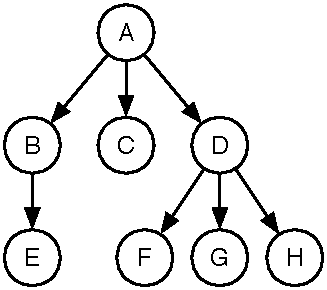
\includegraphics[scale=.75]{binary-search-trees/rootedtree}
\end{center}
\begin{center}
\begin{tabular}{rcl}
root & : & $A$\\
leaves & : & $E$, $C$, $F$, $G$, and $H$\\
internal nodes & : & $A$, $B$, and $D$\\
children of $A$ & : & $B$, $C$ and $D$\\
parent of $E$ & : & $B$\\
descendants of $A$ & : & all nodes, including $A$ itself\\
ancestors of $F$ & : & $F$, $D$ and $A$\\
depth of $F$ & : & 2\\
height of $B$ & : & 1\\
height of the tree & : & 2\\
subtree rooted at $D$ & : & the rooted tree consisting of $D$, $F$, $G$ and $H$
\end{tabular}
\end{center}
\end{example}
\end{figure}

\begin{figure}
\begin{definition}[Binary Tree]
\label{def:binarytree}
A full \emph{binary tree} is an ordered rooted tree in which every node has
exactly two children.  We refer to the first child as the \emph{left
  child} and the second as the \emph{right child}.  The \emph{left
  subtree} of a node is the subtree rooted at the left child, and the
\emph{right subtree} the one rooted at the right child.
\end{definition}

\begin{definition}[Binary Search Tree]
\label{def:bst}
A \emph{binary search tree} (BST) over a totally ordered set $S$ is a
full binary tree that satisfies the following conditions.
\begin{enumerate}
 \item There is a one-to-one mapping $k(v)$ from internal tree nodes to elements in $S$.
 \item for every $u$ in the left subtree of $v$, $k(u) < k(v)$
 \item for every $u$ in the right subtree of $v$, $k(u) > k(v)$
\end{enumerate}
Conditions 2 and 3 are referred to as the \emph{BST property}.  We
often refer to the elements of $S$ in a BST as keys, and use $K(T)$ to
indicate the keys in a BST $T$.  The \emph{size} of a
BST is the number of keys in the tree, i.e. $|S|$.  A BST can
equivalently be defined recursively as:
\[
\cname{BST}(S) = \left\{\begin{array}{ll}
\cname{Leaf} & S = \emptyset\\
\cname{iNode}(\cname{BST}(S_L), k, \cname{BST}(S_R)) & 
\underbrace{(S = S_L \cup \cset{k} \cup S_R)}_{\mbox{one to one (inclusion)}} \wedge \underbrace{(S_L < k < S_R)}_{\mbox{BST property}}
\end{array}\right.
\]
\end{definition}

\begin{example}
\label{ex:bst}
An example binary search tree over the set $\{1,3,4,5,6,7,8,9\}$:
\begin{center}
  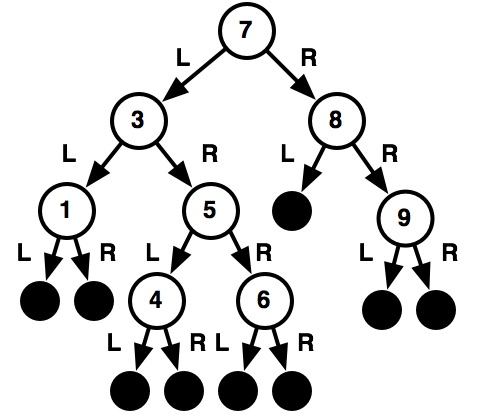
\includegraphics[scale=.75]{binary-search-trees/bst2}~~~~~~~
  \raisebox{.2in}{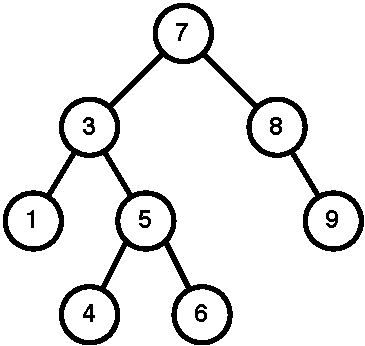
\includegraphics[scale=.75]{binary-search-trees/bst3}}
\end{center}
On the left the $L$ and $R$ indicate the left (first) and right
(second) child, respectively.  All internal nodes (white) have a key
associated with them while the leaves (black) are empty.  The keys
satisfy the BST property---for every node, the keys in the left
subtree are less, and the ones in the right subtree are greater.

\vspace{.05in}

On the right we have dropped the arrows, since we assume edges go
down, the labels $L$ and $R$, since the left and right children will
always be placed on the left and right, respectively, and the leaves,
since they are implied by a missing child.  We use this
convention in future figures.
\end{example}
\end{figure}

\section{The BST Abstract Data Type}

\newcommand{\bstt}{\tttt}
\newcommand{\bstt}{\tttt}

\begin{figure}
\begin{datatype}[\bf BST]
\label{adt:bbst}
\normalsize For a universe of totally ordered keys $\kkk$ and
(possibly unordered) values $\vvv$ the \adt{BBST} is a type $\bstt$
representing key-value pairs.  The BST abstract data type consists of
\bstt and  the following functions.
\[
\begin{array}{lclcl}
\texttt{empty}
& : &\bstt
\\
\texttt{singleton}(k) 
& : & \kkk \rightarrow \bstt
\\
%% \texttt{expose}(T) 
%% & : & \bstt \rightarrow (\cname{Empty}~|~\cname{Node}(\bstt,\kkk,\bstt))
%% \\
\texttt{find}(T,k) 
& : & (\bstt \times \kkk) \rightarrow ((\bbb option) \times \bstt)
\\
\texttt{insert}(T,(k,v)) 
& : & (\bstt \times (\kkk \times \vvv)) \rightarrow  \bstt
\\
\texttt{delete}(T,k) 
& : & (\bstt \times \kkk) \rightarrow  \bstt
\\
\texttt{union}(T_1,T_2)
& : & (\bstt \times \bstt) \rightarrow  \bstt
\\
\texttt{intersection}(T_1,T_2) 
& : & (\bstt \times \kkk) \rightarrow  \bstt
\\
\texttt{split}(T,k) 
& : & (\bstt \times \kkk) \rightarrow (\bstt \times \bbb \times \bstt)
\\
\texttt{join}(T_1,m,T_2) 
& : & (\bstt \times (\cname{Some}(\kkk)~|~\cname{None}) \times \bstt) \rightarrow \bstt 
\\
\end{array}
\]
\end{datatype}
\end{figure}

Abstract Data Type~\ref{adt:bbst} describes an ADT for balanced BSTs
based on split and join.  In addition to \cname{split} and
\cname{join} the interface supplies an empty tree, a function for
building a singleton tree, and a function \cname{expose} that exposes
the root of the tree by returning its left and right branches and its
key.  The reason the interface uses \cname{expose} instead of giving
direct access to the tree node is to abstract away from the particular
balancing scheme.  The balancing scheme might contain additional
information in the nodes, such as the height of the tree, or a color.


--


\paragraph{Searching with a BST.}
The main idea behind binary search trees is that the keys on the
internal nodes allow us to find if a given key is in the tree  by
taking a single path through the tree.  In particular for a key $k$ we
can start at the root $r$ and if $k$ equals the key at the root,
$k(r)$, then we have found our key, otherwise if $k < k(r)$, then we
know that $k$ cannot appear in the right subtree, so we only need to
search the left subtree, and if $k > k(r)$, then we only have to
search the right subtree.  Continuing the search we will either find
the key or reach a leaf and determine the key is not in the tree.  In
both cases we have followed a single path through the BST starting at
the root.   We can write the algorithm for finding a key in 
a BST as follows.

\begin{algorithm}[Finding a key in a BST]~
\begin{lstlisting}[numbers=none]
fun find$(T,k)$ =
  case $T$ of 
     Leaf => False
   | iNode$(L,k',R)$ => 
       case compare$(k,k')$ of
          Less => find$(L,k)$
        | Equal => true
        | Greater => find$(R,k)$
\end{lstlisting}
\end{algorithm}

This form of search in a BST can be generalized beyond binary trees to
work with tree nodes with higher degrees.  To do this, for a node with
$k$ children, we would need $k-1$ keys so separate each of the
children.  In this book we only cover binary search trees.

\paragraph{A Balancing Act.}
Since a \cname{find} only follows a path in the BST, and assuming the
comparison at each step takes constant work, it takes work at most
proportional to the height of the tree.  Therefore, if we want to find
keys quickly, we need to ensure that the height of the tree is small.
A binary tree is defined to be \emph{perfectly balanced} if it has the
minimum possible height.  For a binary search tree over a set $S$, a
perfectly balanced tree has height exactly $\lceil \log_2 (|S| + 1) \rceil$.
\begin{exercise}
Prove that the minimum possible height of a binary search tree
with $n$ keys is $\lceil \log_2 (n + 1)\rceil$.
\end{exercise}
Ideally we would use a perfectly balanced tree.  Indeed if we never
make changes to the tree, we could balance it once up front and it
would remain balanced.  However, if we want to update the tree by, for
example, inserting new keys or combining two trees, then maintaining
such perfect balance is costly.  It turns out to be impossible, for
example, to maintain a perfectly balanced tree while allowing
insertions in $O(\log n)$ work.  BST data structures therefore aim to
keep approximate or near balanced instead of perfect balance.  We
refer to a BST data structure as {\em balanced} or {\em near balanced}
if all trees with $n$ elements have height $O(\log n)$, perhaps in
expectation or with high probability.

There are many balanced BST data structures.  Most either try to
maintain height balance (the children of a node are about the same
height) or weight balance (the children of a node are about the same
size).  Here we list a few such data structures:

\begin{enumerate}
\item \emph{AVL trees}  are the earliest near-balance BST data
  structure (1962).  It maintains the invariant that the two children
  of each node differ in height by at most one, which in turn implies
  near balance.

\item \emph{Red-Black trees} maintain the invariant that all leaves
  have a depth that is within a factor of 2 of each other.  The depth
  invariant is ensured by a scheme of coloring the nodes red and
  black.

\item \emph{Weight balanced (BB[$\alpha$]) trees} maintain the
  invariant that the left and right subtrees of a node of size $n$
  each have size at least $\alpha n$ for $0 < \alpha \leq
  \frac{1}{2}$.  The BB stands for bounded balance, and adjusting
  $\alpha$ gives a tradeoff between search and update costs.

\item \emph{Treaps} associate a random priority with every key and
  maintain the invariant that the keys are stored in heap order with
  respect to their priorities (treaps is short for tree-heaps).
  Treaps guarantee near balance with high-probability.

\item \emph{Splay trees} are an amortized data structure that does not
  guarantee near balance, but instead guarantees that for any sequence
  of $m$ insert, find and delete operations each does $O(\log n)$
  amortized work.
\end{enumerate}
There are dozens of other balanced BST data structures (e.g. scapegoat
trees and skip lists), as well as many that allow larger degrees,
including 2--3 trees , brother trees, and B trees.  In this chapter we
will cover treaps, red-black trees, and briefly AVL trees.

\section{Split and Join}

%%%% Repetition
%% Traditionally treatments of binary search trees concentrate on three
%% operations \cname{find}, \cname{insert}, and \cname{delete}.  Out of
%% these, \cname{find} is naturally parallel since any number of searches
%% can proceed in parallel with no conflicts\footnote{In splay trees and
%%   other self-adjusting trees, this is not true since a search can
%%   modify the tree.}. Insert and delete, however, are inherently
%% sequential since they update a tree one element at a time.  For this
%% reason, 

We describe two functions, \textbf{split} and \textbf{join}, for
operating on BST's.  These function, which respectively split a BST
into two and to join two BST's, can be used to implement many
operations on BST's, including parallel insertions and deletions.

%% The functions \textbf{split} and \textbf{join} can be used to
%% implement parallel algorithms for functions such as \cname{union},
%% \cname{intersection} and \cname{difference}, and their counterparts on
%% tables (\cname{merge}, \cname{extract}, \cname{erase}).

%In the following discussion $\kkk$ indicates the
%totally ordered universe of keys we are working over.

\begin{comment}
We are interested in two functions, called \cname{split}
and \cname{join}, with the following types:
\begin{lstlisting}[numbers=none]
  split$(T,k)$ : BST ** $\kkk$ -> BST ** $\bbb$ ** BST@\vspace{.1in}@
  join$(T_1,m,T_2)$ : BST ** ($\kkk$ option) ** BST -> BST 
\end{lstlisting}
where $\bbb$, as usual, indicates a Boolean.
\end{comment}

The \cname{split}$(T,k)$ function splits the tree $T$ by the key $k$,
returning two trees, one with all the keys in $T$ less than $k$,
and the other with all the keys greater than $T$.   It also returns a
Boolean indicating whether $k$ appears in $T$.
\begin{example}
Two examples of the split operation.
\[\cname{split}\left(
\raisebox{-.45in}{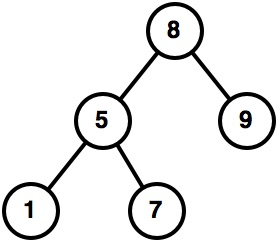
\includegraphics[scale=.6]{binary-search-trees/bst4}}~~,
~~6\right) \Rightarrow \left(
\raisebox{-.27in}{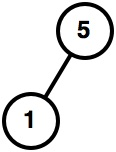
\includegraphics[scale=.6]{binary-search-trees/bst4a}}~~,
~\cname{False}~,~~
\raisebox{-.27in}{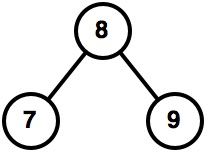
\includegraphics[scale=.6]{binary-search-trees/bst4b}}
\right) 
\]
\[\cname{split}\left(
\raisebox{-.45in}{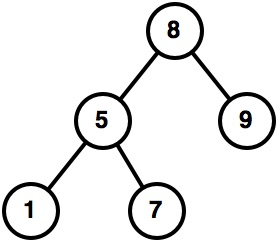
\includegraphics[scale=.6]{binary-search-trees/bst4}}~~,
~~5\right) \Rightarrow \left(
\raisebox{-.1in}{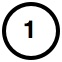
\includegraphics[scale=.6]{binary-search-trees/bst4c}}~~,
~\cname{True}~,~~
\raisebox{-.27in}{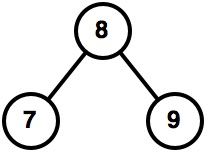
\includegraphics[scale=.6]{binary-search-trees/bst4b}}
\right) 
\]
\end{example}
The \cname{join}$(T_1,m,T_2)$ function takes two trees and an optional
key $m$.  If $m$ contains key $k$, then we require that $K(T_1) < k <
K(T_2)$, otherwise we require that $K(T_1) < K(T_2)$.  The function joins
all the values into a single tree.
\begin{example}
An example of the join operation:
\[\cname{join}\left(
\raisebox{-.27in}{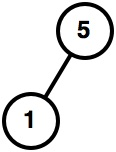
\includegraphics[scale=.6]{binary-search-trees/bst4a}}~~,
~~\cname{None}~~,
~~\raisebox{-.27in}{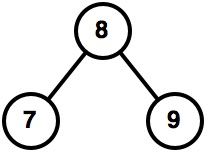
\includegraphics[scale=.6]{binary-search-trees/bst4b}}
\right) \Rightarrow
\raisebox{-.45in}{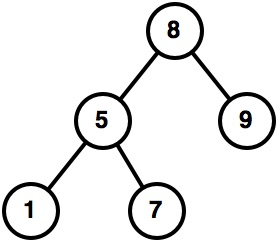
\includegraphics[scale=.6]{binary-search-trees/bst4}}
\]
\[\cname{join}\left(
\raisebox{-.1in}{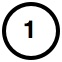
\includegraphics[scale=.6]{binary-search-trees/bst4c}}~~,
~~\cname{Some}(5)~~,
~~\raisebox{-.27in}{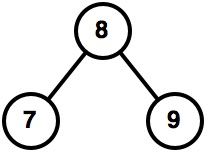
\includegraphics[scale=.6]{binary-search-trees/bst4b}}
\right) \Rightarrow
\raisebox{-.45in}{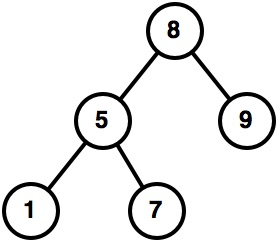
\includegraphics[scale=.6]{binary-search-trees/bst4}}
\]
The result of the join could have different tree structures, but it
must be a valid BST and contain the union of the keys.  In the second
case, for example, the $5$ could be at the root with the tree containing $1$ as its
left child.
\end{example}

The structure of the trees returned by \cname{split} and \cname{join}
depend on the balancing scheme.  The \cname{split} and \cname{join}
for a particular scheme are required required to maintain the
balance---i.e., if the input trees satisfy the conditions of that
scheme, then the output must also.  For example, a \cname{split}
designed for red-black trees (discussed later), must, if given a
red-black tree, return two red-black trees.  As we will see, the
algorithms for \cname{split} and \cname{join} on near-balanced trees
can be implemented to run in $O(\log n)$ work.

\begin{figure}
\begin{algorithm}[FInd, Insert and Delete using Split and Join]~
\label{alg:searchInsertDelete}
\begin{lstlisting}[numbers=none]
function find$(T,k)$ =
  let val (_,$v$,_) = split$(T,k)$
  in $v$ end @\vspace{.15in}
@
function insert$(T,(k,v))$ =
  let val $(L, \_, R)$ = split$(T,k)$
  in join$(L,\cname{Some}(k,v),R)$ end @\vspace{.15in}
@
function delete$(T,k)$ =
  let val $(L, \_, R)$ = split$(T,k)$
  in join$(L, \cname{None}, R)$ end
\end{lstlisting}
\end{algorithm}
\end{figure}

With \cname{split} and \cname{join}, we can easily implement
\sml{find}, \sml{insert}, and \sml{delete} as shown in
Algorithm~\ref{alg:searchInsertDelete}.  Since these functions make at
most two calls to \cname{split} and \cname{join}, they will also take
$O(\log n)$ work.  This is asymptotically optimal in the comparison
model---just finding the key takes $\Omega(\log n)$ work.  
Direct implementations, however, might be a constant factor faster.


\begin{figure}
\begin{datastructure}[Implementing \adt{balancedBST} with no balance criteria]~
\label{ds:bstjoin}
\begin{lstlisting}
datatype $\tttt$ = Empty | Node of ($\tttt$ ** $\kkk$ ** $\tttt$)@
\vspace{.1in}@
val empty = Empty@
\vspace{.1in}@
function singleton$(k)$ = Node(Empty,$k$,Empty)@
\vspace{.1in}@
function expose$(T)$ = $T$@
\vspace{.1in}@
function split$(T,k)$ =
  case expose$(T)$ of
    Empty => (Empty, False, Empty)
  | Node$(L,k',R)$ =
      case compare$(k,k')$ of
        LESS => @\label{line:split-less}@
          let val $(L',m',R')$ = split$(L,k)$
          in $(L',m',\cname{Node}(R',k',R))$ end @\label{line:splitnode1}@
      | EQUAL => $(L,~\cname{True},R)$
      | GREATER => @\label{line:split-greater}@
          let val $(L',m',R')$ = split$(R,k)$
          in (Node$(L,k',L'),m',R'$) end @\label{line:splitnode2}@@
\vspace{.1in}@
function join$(T_1,m,T_2)$ =
  case $m$ of
    Some$(k)$ => Node$(T_1,k,T_2)$
  | None =>
      case $T_1$ of
        Empty => $T_2$
      | Node$(L,k,R)$ => Node$(L,k,~\cname{join}(R,\cnone,T_2)))$@
\end{lstlisting}
\end{datastructure}
\end{figure}

\paragraph{BSTs without balance.}
If we do not care about balance, then the BST interface is reasonably easy
to implement, and is given in Data Structure~\ref{ds:bstjoin}.    
The \cname{split} algorithm recursively traverses the tree from the
root to the key $k$ splitting along the path, and then when returning from
the recursive calls, it puts the subtrees back together.
\begin{example}
In the following tree we split on the key $c$, which does not appear
in the tree.  The split traverses
the path $\cseq{a,e,b,d}$ turning right at $a$ and $b$
(line~\ref{line:split-greater} of the Data Structure~\ref{ds:bstjoin})
and turning left at $e$ and $d$ (line~\ref{line:split-less}).  The
pieces are put back together into the two resulting trees on the way
back up the recursion.  
\begin{center}
  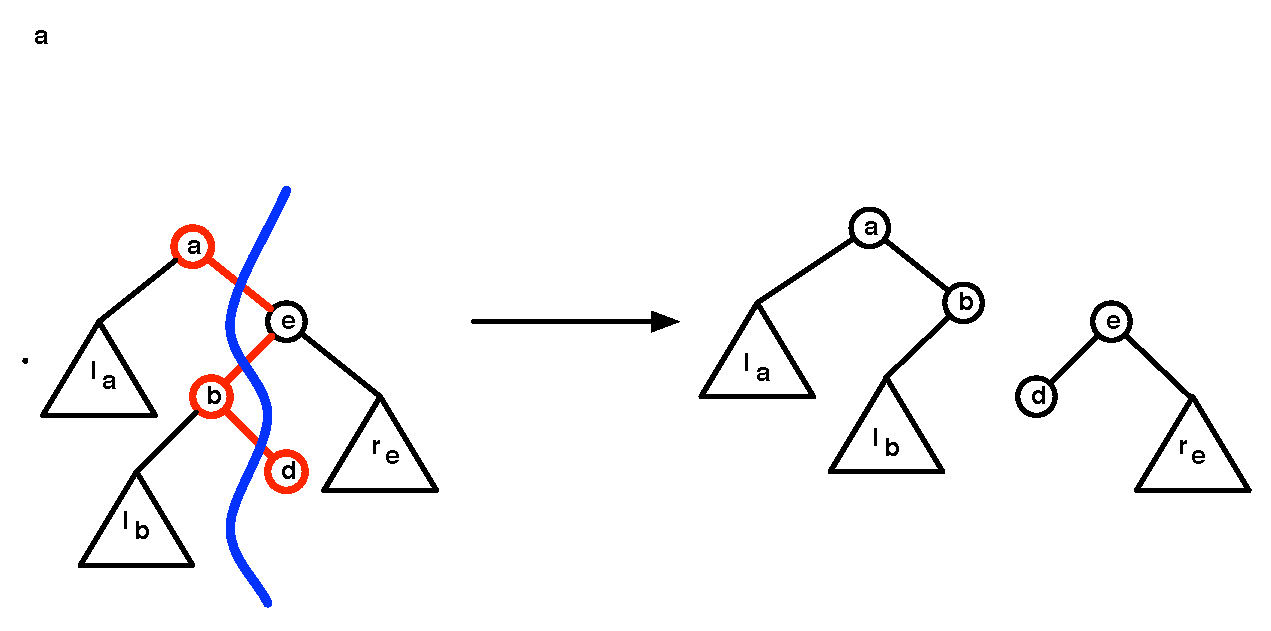
\includegraphics[width=5.7in]{binary-search-trees/bstsplit}
\end{center}
%The actual way the trees will be put back together will depend on the
%balancing scheme.
\end{example}
The \cname{join} algorithm with a key in the middle simply calls
\cname{Node} and therefore does constant work.  For near-balanced
trees, however, \cname{join} needs to rebalance the tree and can take
work proportional to the height of the trees.

\begin{example}
Using the version of \cname{join} with no rebalancing (from Data Structure~\ref{ds:bstjoin})
we have:
\[\cname{join}\left(
\raisebox{-.45in}{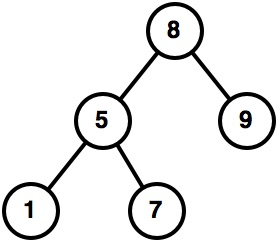
\includegraphics[scale=.6]{binary-search-trees/bst4}}~~,
~\cname{Some}(10)~,
~\cname{Empty}
\right) \Rightarrow 
\raisebox{-.7in}{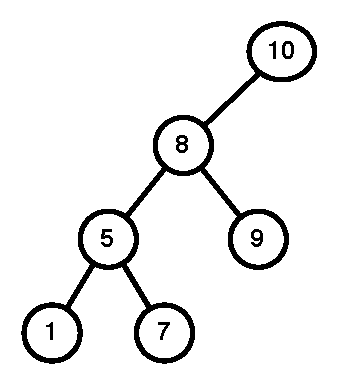
\includegraphics[scale=.6]{binary-search-trees/bst4d}}
\]
The resulting tree is clearly not balanced since we joined a tree of
height three with one of height zero and did no rebalancing.  The join
in a near-balanced scheme needs to rebalance the tree, as we will see
later.
\end{example}

\paragraph{Minimal Interface.}
We refer to a join that always takes a key in the middle
\cname{joinMid}$(L,k,R)$ and one that never takes a key as
\cname{joinPair}$(L,R)$.  It turns out that we only need one of these
and the other can be efficiently implemented using it.  For
example:
\begin{lstlisting}[numbers=none]
joinMid$(L,k,R)$ = joinPair($L$,joinPair(singleton($k$),R)
\end{lstlisting}
\begin{exercise}
Implement \cname{joinPair} with \cname{joinMid} and any other
functions in the balancedBST ADT.
\end{exercise}
It is also possible to implement \cname{split} efficiently with
\cname{join}.  Indeed the algorithm for such a split is the same code
as in Data Structure~\ref{ds:bstjoin}, except that the
\cname{Node} on Lines~\ref{line:splitnode1} and~\ref{line:splitnode2}
replaced with \cname{joinMid}.
This implies that to achieve a new asymptotically efficient
implementation of a near balanced BST scheme, all one needs to
implement is one of \cname{joinMid} or \cname{joinPair}, along with
supplying \cname{expose} and \cname{empty} (\cname{singleton}$(k)$ is
easily defined as \cname{joinMid(empty,$k$,empty)}).  

\begin{comment}
\begin{exercise}
Write a version of \cname{insert} that takes a function $f : \data
\times \data$ and if the insertion key $k$ is already in the tree
applies $f$ to the old and new value to return the value to associate
with the key.
\end{exercise}
\end{comment}

\section{Union, Intersection and Difference}
\label{sec:union}

Let us now consider a more interesting operation: taking the
\cname{union} of two BSTs.  Note that this differs from $\cjoin$ since
we do not require that all the keys in one tree appear before the
keys in the other tree.  To implement \cname{union}$(T_1,T_2)$ in
parallel we use a divide-and-conquer approach.  The idea is to split
both trees based on some key $k$, recursively union the two parts with
keys less than $k$, and the two parts with keys greater than $k$ and
then join them.  How do we find the key $k$?  One way is simply to use
the key at the root of one of the two trees, for example the first tree,
and split the second tree with it.
\begin{example}
\cname{union}$(T_1,T_2)$ by using the key $k_1$ at the root of $T_1$ to
split $T_2$ and recursively unioning the parts less than $k_1$ and the
parts greater than $k_1$.
\begin{center}
  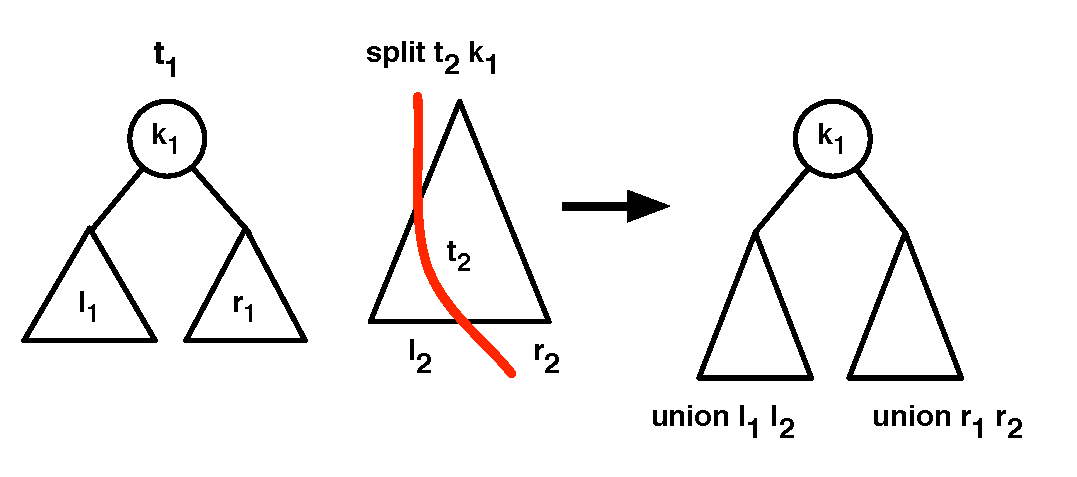
\includegraphics[scale=.7]{binary-search-trees/union-dia1}
\end{center}
\label{example:tree-union}
\end{example}
This idea leads to Algorithm~\ref{alg:union}.  
%For simplicity, this
%version returns the value from $T_1$ if a key appears in both BSTs,
Notice that \cname{union} only uses the functions in our
\adt{balancedBST} interface and therefore can be used for any near
balanced binary tree implementing that interface.  The algorithm for
\cname{intersect} is very similar and is given in
Algorithm~\ref{alg:intersect}.  We now analyze the cost of
\cname{union} (and \cname{intersect}).

\begin{figure}
\begin{algorithm}[Union of two BSTs]~
\label{alg:union}
\begin{lstlisting}
function union$(T_1, T_2)$ =
  case (expose$(T_1)$,expose$(T_2)$) of
    (Empty,_) => $T_2$
  | (_,Empty) => $T_1$
  | (Node$(L_1,k_1,R_1)$,_) =>
      let 
        val $(L_2, \_, R_2)$ = split$(T_2,k_1)$
        val $(L,R)$ = (union$(L_1,L_2)$ || union$(R_1, R_2)$)
      in 
        join$(L,~\csome(k_1),~R)$
      end
\end{lstlisting}
\end{algorithm}
\end{figure}

\begin{figure}
\begin{algorithm}[Intersection of two BSTs]~
\label{alg:intersect}
\begin{lstlisting}
function intersect$(T_1, T_2)$ =
  case (expose$(T_1)$,expose$(T_2)$) of
    (Empty,_) => Empty
  | (_,Empty) => Empty
  | (Node$(L_1,k_1,R_1)$,_) =>
      let 
        val $(L_2, b, R_2)$ = split$(T_2,k_1)$
        val $(L,R)$ = (intersect$(L_1,L_2)$ || intersect$(R_1, R_2)$)
      in 
        join($L$, if $b$ then Some$(k_1)$ else None, $R$)
      end
\end{lstlisting}
\end{algorithm}
\end{figure}

% We note, however, that as written the code only matches our desired bounds if
% $|T_1| \leq |T_2|$.
%
%



\subsection*{Cost of Union}

As described in Chapter~\ref{ch:sets-tables}, \cunion{} and similar
functions (e.g., \cname{intersection} and \cname{difference} on sets
and \cname{merge}, \cname{extract} and \cname{erase} on tables) have
expected $O(m \log (1 + \tfrac{n}m))$ work, where $m$ is the size of
the smaller input and $n$ the size of the larger one.
%This bound is the same as the lower bound for merging two sorted
%sequences.
We will see how
this bound falls out very naturally from the \sml{union} code.

To analyze \cname{union}, we assume that the work and span of
\csplit{} on a tree of size $n$ and \cjoin{} returning a tree of size
$n$ take $O(\log n)$ work.  This is true for near balance schemes, as
we will see for treaps and red-black trees.
To ease the analysis, we will make the following assumptions:
\begin{enumerate}
\item $T_1$ it is perfectly balanced (i.e., \cexpose{} returns subtrees of
  size at most $|T_1|/2$), 
\item Each time a key from $T_1$ splits $T_2$, it splits the tree in
  exactly in half, and
\item without loss of generality let $|T_1| \leq |T_2|$.
\end{enumerate}
Later we will relax these assumptions.  Let us define $m = |T_1|$ and
$n = |T_2|$ (recall the size of a tree is the number of keys in it).
With these assumptions and examining the algorithm we can then write
the following recurrence for the work of \cname{union}:
\begin{align*}
  W_{\mbox{union}}(m, n) &\leq 2W_{\mbox{union}}(m/2,n/2) + W_{\mbox{split}}(n)
+ W_{\mbox{join}}(n+m) + O(1)\\
   & \leq  2W_{\mbox{union}}(m/2, n/2) + O(\log n)~.
\end{align*}  
The size for join is the sum of the two sizes, $m+n$, but since 
$m \leq n$, $O(\log (n + m))$ is equivalent to $O(\log n)$.
We also have the base case
\begin{align*}
  W_{\mbox{union}}(1, n) & \leq 2W_{\mbox{union}}(0,n/2) + W_{\mbox{split}}(n)
+ W_{\mbox{join}}(n) + O(1)\\
         & \leq O(\log n)~.
\end{align*}
The final inequality is since $2W_{\mbox{union}}(0,n) = O(1)$.

If we draw the recursion tree that shows the work associated with
splitting $T_2$ and joining the results, we obtain the following:

%This figure should be changed so "n" is replaced by "N" except the
%bottom level should be "each costs log (1 + n/m)"

\begin{center}
  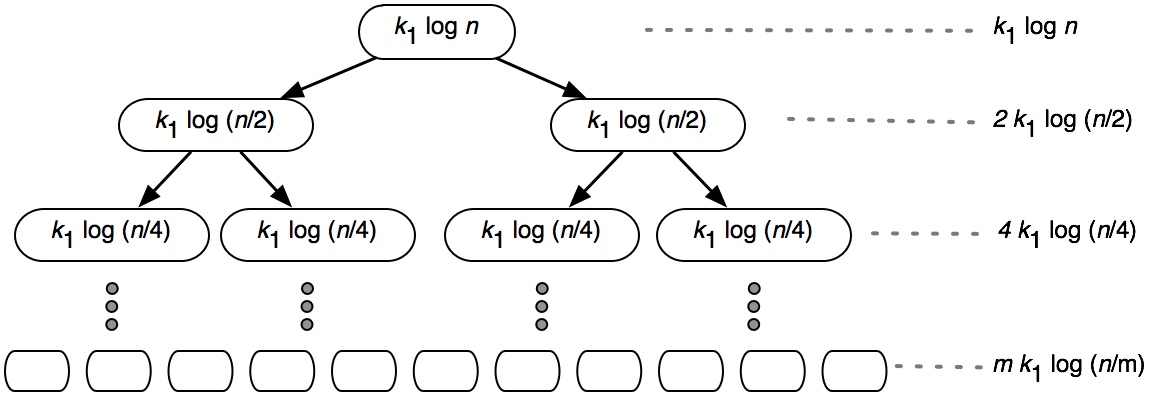
\includegraphics[scale=.65]{binary-search-trees/recurtree2}
\end{center}
%
There are several features of this tree that's worth mentioning:
First, ignoring the somewhat-peculiar cost in the base case, we know
that this tree is leaf-dominated.  Therefore, excluding the cost at
the bottom level, the cost of \cunion{} is $O(\#\text{ of leaves})$
times the cost of each leaf.

\emph{But how many leaves are there? And how deep is this tree?}  To
find the number of leaves, we will take a closer look at the work
recurrence.  Notice that in the recurrence, the tree bottoms out when
$m = 1$ and before that, $m$ always gets split in half (remember
that $T_1$ is perfectly balanced).  Nowhere in there does $T_2$
affects the shape of the recursion tree or the stopping condition.
Therefore, this is yet another recurrence of the form $f(m) = f(m/2) +
O(...)$, which means that \emph{it has $m$ leaves and is $(1 + \log_2
  m)$ deep.}

Next, we will determine the size of $T_2$, i.e. $n$, at the leaves.
Well we had $m$ keys in $T_1$ to start with, and they chopped $T_2$
evenly, so each part at the base case will have size $\frac{n}{m}$.
Therefore, each leaf node costs $O(\log (1+\frac{n}{m}))$ (the $1+$ is
needed to deal with the case that $n = m$).  Since there are $m$
leaves, the whole bottom level costs $O(m \log (1+ \frac{n}{m}))$.
Hence, if the trees satisfy our assumptions, we have that \cunion{}
runs in $ O( m\log(1 + \frac{n}{m}))$ work.

\paragraph{Removing An Assumption:} Of course, in reality, our keys in $T_1$
won't split subtrees of $T_2$ in half every time.  But it turns out
that any unevenness in the splitting only helps reduce the
work---i.e., the perfect split is the worst case.  We won't go through
a rigorous argument, but if we keep the assumption that $T_1$ is
perfectly balanced, then the shape of the recursion tree stays the
same.  What is now different is the cost at each level.  Let us try to
analyze the cost at level $i$.  At this level, there are $k = 2^i$
nodes in the recursion tree. Say the sizes of $T_2$ at these nodes are
$n_1, \dots, n_k$, where $\sum_j n_j = n$. Then, the total cost for
this level is
\[
c \cdot \sum_{j=1}^k \log (n_j) \;\;\leq\;\; c \cdot \sum_{j=1}^k \log (n/k) =
c\cdot 2^i \cdot \log (n/2^i),
\]
where we used the fact that the logarithm function is
concave\footnote{Technically, we're applying the so-called Jensen's
  inequality.}.  Thus, the tree remains leaf-dominated and the same
reasoning shows that the total work is $O(m \log (1 + \frac{n}{m}))$.

Still, in reality, $T_1$ doesn't have to be perfectly balanced as we
assumed. A similar reasoning can be used to show that $T_1$ only has
to be approximately balanced. We will leave this case as an exercise.
We end by remarking that as described, the span of \cunion{} is
$O(\log^2 n)$, but this can be improved to $O(\log n)$ by changing the
algorithm slightly.

In summary, \cunion{} can be implemented in $O(m \log (1 +
\tfrac{n}m))$ work and span $O(\log n)$.  The same holds for the other
similar operations (e.g. \cname{intersection}).

\section{Treaps}

The first scheme we consider for maintaining nearly balanced is
treaps.  Treaps are likely the simplest of all the schemes, but they
are randomized and hence they only guarantee near balance with high
probability.  The idea behind the scheme is to assign a priority to
each key and keep the priorities in heap order---the priority of each
node is larger than that of its children.  More formally:

\begin{definition}[Treap]
A treap is a binary search tree $T$ over a set $S$ along with 
a \emph{priority} for each key given by \[p : \kkk \rightarrow \zzz~,\] that
in addition to satisfying the BST property on the keys $S$, satisfies the 
heap property on the priorities $p(s), s \in S$, i.e., for every node $v$:
\[p(k(v)) \geq p(k(L(v))) \mbox{ and } p(k(v)) \geq p(k(R(v)))\]
\end{definition}

\begin{example}
The following key-priority pairs $(k,p(k))$, 
\[ (a,3), (b,9), (c, 2), (e,6), (f, 5)~,\] where the keys are ordered
alphabetically, form the following treap:
\begin{center}
  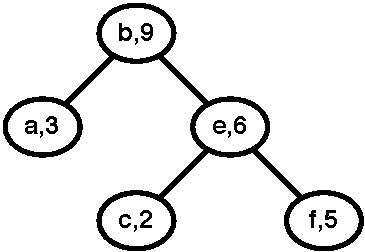
\includegraphics[width=2in]{binary-search-trees/treap-examp}
\end{center}
since $9$ is larger than $3$ and $6$, and $6$ is larger than $2$ and
$5$.
\end{example}
\begin{exercise}
Prove that if the priorities are unique, then there is exactly one tree
structure that satisfies the treap properties.
\end{exercise}

So how do we assign priorities?  It turns out that if the priorities are
selected randomly then the tree is guaranteed to be near balanced,
i.e. $O(\log |S|)$ height, with high probability.  We will get back to
showing this shortly, but for now let us first implement \cname{split}
and \cname{join}, and show that the work for the functions
are asymptotically bounded by the height of the tree.  We 
also give a direct implementation of \cname{insert}.

\begin{figure}
\begin{datastructure}[Implementing \adt{balancedBST} with treaps]~
\label{ds:treapjoin}
\begin{lstlisting}
datatype $\tttt$ = Empty | Node of ($\tttt$ ** $\kkk$ ** $\tttt$)@
\vspace{.1in}@
val empty = Empty@
\vspace{.1in}@
function singleton$(k)$ = Node(Empty,$k$,Empty)@
\vspace{.1in}@
function expose$(T)$ = $T$@
\vspace{.1in}@
function split$(T,k)$ = % Same as in Data Structure @\ref{ds:bstjoin}@@\vspace{.1in}@
function join$(T_1,m,T_2)$ =
let
  fun joinPair$(T_1,T_2)$ =
    case $(T_1,T_2)$ of
      (Leaf , _) => $T_2$
    | (_ , Leaf) => $T_1$
    | (Node$(L_1,k_1,R_1)$, Node$(L_2,k_2,R_2)$) =>
       if ($p(k_1) > p(k_2)$) then @\label{line:cpri}@
         Node($L_1$, $k_1$, joinPair$(R_1,T_2)$)
       else
         Node(joinPair$(T_1,L_2)$, $k_2$, $R_2$)
in
  case $m$ of
    None => joinPair$(T_1, T_2)$
  | Some$(k)$ => joinPair($T_1$, joinPair(singleton$(k)$, $T_2$))
end
\end{lstlisting}
\end{datastructure}
\end{figure}

The implementation of \adt{balancedBST} (\cname{singleton},
\cname{expose}, \cname{split} and \cname{join}) using treaps is given
in Data Structure~\ref{ds:treapjoin}.  The code for \cname{split} is
unchanged from the version that did not maintain balance (Data
Structure ~\ref{ds:bstjoin}).  This is because when using
$\cname{Node}$ on Lines~\ref{line:splitnode1}
and~\ref{line:splitnode2}, the priority of the key $k'$ is the highest
priority key in the input tree $T$ and is therefore larger than the
priorities of either of the subtrees on the left and right.  Hence
\cname{split} will maintain the heap property of treaps.

However, the algorithm for \cname{join}$(L,k,R)$ needs to be changed
since the version with no rebalancing places $k$ at the root, which
does not necessarily have a higher priority than the roots of $L$ and
$R$.  The heap property might therefore needs to be fixed.  The data
structure uses \cname{joinPair} to implement \cname{join}.  In
\cname{joinPair} we first compare the priorities of the two roots,
making the larger priority the new root.   We then can recursively join the pair consisting of the
other tree and the appropriate side of the new root.    This is
illustrated in the following example:
\begin{example}
\label{ex:treap-join}
\cname{joinPair}$(T_1,T_2)$ on treaps.  If $p(k_1) >
p(k_2)$ we recur with $\cname{joinPair}(R_1,T_2)$
and the result becomes the right child of $k_1$.
\begin{center}
  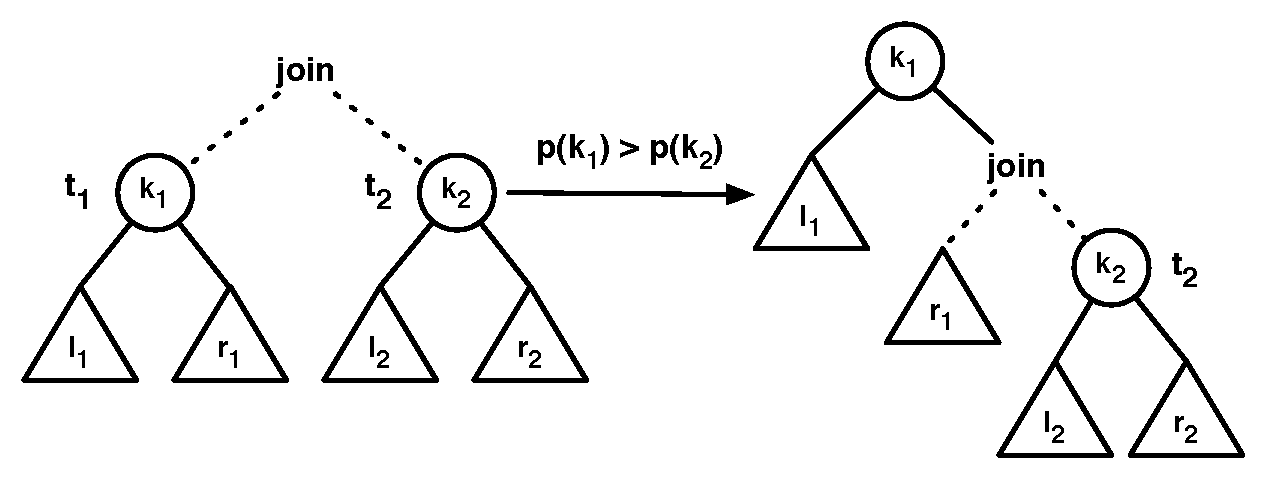
\includegraphics[scale=.6]{binary-search-trees/treap-join}
\end{center}
\end{example}
The path from the root to the leftmost node in a BST is
called the \emph{left spine}, and the path from the root
to the rightmost node is called the \emph{right spine}.   What
$\cname{joinPair}(T_1,T_2)$ does is merge the right spine of $T_1$ with the
left spine of $T_2$ based on the priority order.  This ensures that
the priorities are in decreasing order down the path.
\begin{example}
\cname{joinPair}$(T_1,T_2)$ on treaps in more detail.  The right
spine of $T_1$ consisting of $(b,9)$, $(d,6)$ and $(e,5)$ is merged by
priority with the left spine of $T_2$ consisting of $(h,8)$ and
$(g,4)$.  Note that splitting the result with the key $f$ will return the
original two trees.
\begin{center}
  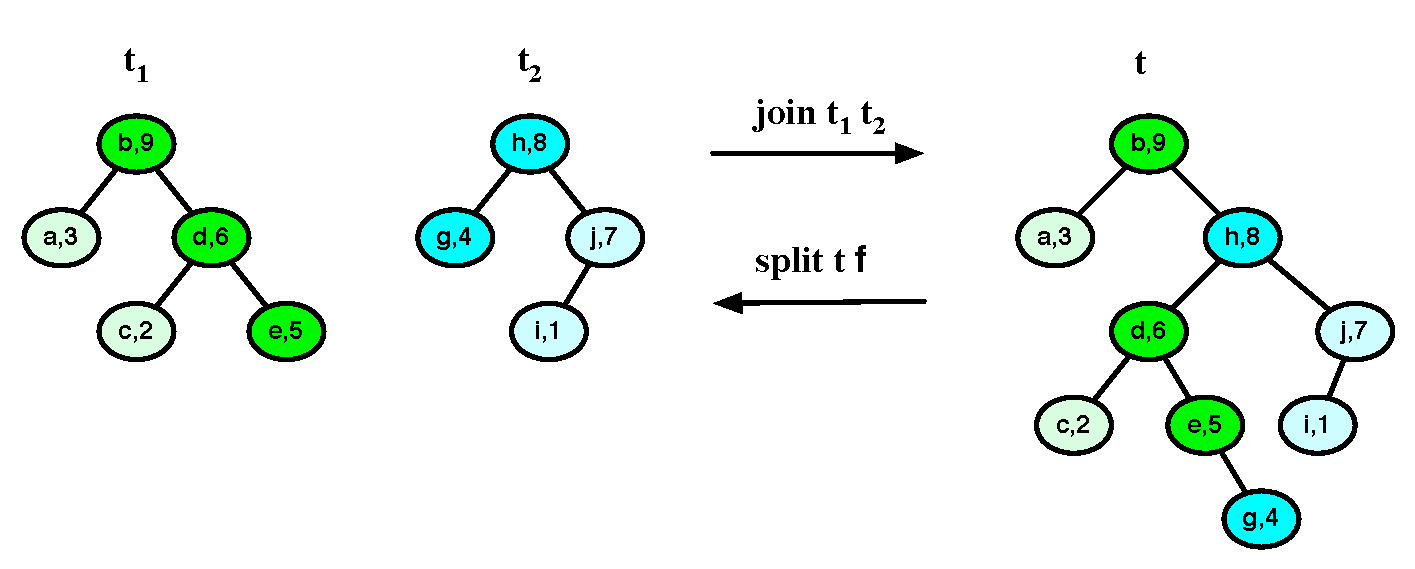
\includegraphics[width=5.8in]{binary-search-trees/treap-examp-join}
\end{center}
\end{example}

\begin{figure}
\begin{algorithm}[Insertion into a Treap]~
\label{alg:treapJoin}
\begin{lstlisting}
function rotateRight$(\cname{Node}(L_l,k,L_r),k',R)$ =
  if $(k > k')$ then Node$(L_l,k,\cname{Node}(L_r,k',R))$  % rotate right
  else Node$(\cname{Node}(L_l,k,L_r),k',R)$           % leave as is@\vspace{.1in}@
function insert$(T,k)$ =
   case $T$ of
     Leaf => singleton$(k)$
   | Node$(L,k',R)$ => 
       case compare$(k,k')$ of
          Less => rotateRight(insert$(L,k),k',R$)
        | Equal => Node$(L,k,R)$
        | Greater => rotateLeft($L,k'$,insert$(R,k)$)
\end{lstlisting}
\end{algorithm}
\end{figure}

\begin{comment}
\begin{lemma}
\label{thm:treapuniqueness}
  For a set of keys $S$, if their priorities $p(s) : s \in S$ are unique,
  then there is exactly one treap (i.e. shape) for $S$.

\begin{proof} (By induction on size)
An empty tree is a leaf (base case).  Otherwise, the unique key $k$
with the highest priority in $S$ must be at the root.  This fixes the
keys to the left ($\csetf{k' \in S}{k' < k}$) and to the right
($\csetf{k' \in S}{k' > k}$).  By induction these are unique, so the
whole tree is unique.
\end{proof}
\end{lemma}
\end{comment}

We are now interested in the work for split and join.  Each one does
constant work on each recursive call.  For \cname{split} each
recursive call goes to one of the children, so the number of recursive
calls is at most the height of $T$.  For \cname{join} each recursive
call either goes down one level in $T_1$ or one level in $T_2$.
Therefore the number of recursive calls is bounded by the sum of the
heights of the two trees.  Hence the work of \cname{split}$(T,k)$ is
$O(h(T))$ and the work of \cname{join}$(T_1,m,T_2)$ is
$O(h(T_1)+h(T_2))$.  This leaves us with the question of what is the
height of a treap?

\paragraph{Analysis of randomized treaps.}   We now analyze the height
of a treap assuming that the priorities are picked at random.     To
do this we will relate treaps to quicksort, which we analyzed in
Chapter~\ref{ch:randomized}.
In particular consider the following variant of quicksort.
\begin{algorithm}{Treap Generating Quicksort}~
\begin{lstlisting}
function qsTree$(S)$ =
  if $|S| = 0$ then Leaf
  else let
    val pivot = @\rm the key $k \in S$ for which $p(k)$ is the largest@
    val $S_1$ = $\cseqf{s \in S}{s < \mbox{pivot}}$
    val $S_2$ = $\cseqf{s \in S}{s > \mbox{pivot}}$
    val $(L, R)$ = (qsTree$(S_1)$ || qsTree$(S_2)$)
  in
    Node$(L, \mbox{pivot}, R)$@\label{alg:qsnode}@
  end
\end{lstlisting}
\end{algorithm}
This algorithm is almost identical to our previous quicksort except that it
uses \cname{Node} instead of \cname{append} on line \ref{alg:qsnode},
\cname{Leaf} instead of an empty sequence in the base case, and, since
it is generating a set, it needs only keep one copy of the keys equal
to the pivot.

The tree generated by \cname{qsTree}$(S)$ is the treap for $S$.  This
can be seen by induction.  It is true for the base case.  Now assume
by induction it is true for the trees returned by the two recursive
calls.  The tree returned by the main call is then also a treap since
the \cname{pivot} has the highest priority, and therefore is correctly
placed at the root, the subtrees and in heap order by induction, and
because the keys in $T_L$ are less than the pivot, and the keys in
$T_R$ are greater than the pivot, the tree has the BST property.

What does this tell us about the height of treaps?  Well it tells us
that the height of a treap is identical to the recursion depth of
quicksort.  In Chapter~\ref{ch:randomized} we proved that if we pick
the priorities at random, the recursion depth is $O(\log n)$ with high
probability.  Therefore we know that the height of a treap is $O(\log
n)$ with high probability.

\begin{comment}
\section{Expected Depth of a Key in a Treap}

Consider a set of keys $K$ and associated priorities $p : \cname{key}
\rightarrow \cname{int}$.  For this analysis, we assume the priorities
are unique and random.  Consider the keys laid out in order, and as
with the analysis of quicksort, we use $i$ and $j$ to refer to the
$i^{th}$ and $j^{th}$ keys in this ordering.  Unlike quicksort
analysis, though, when analyzing the depth of a node $i$, $i$ and $j$ can
be in any order, since an ancestor of $i$ in a BST can be either less than or
greater than $i$.

\begin{verbatim}
     | | | | | | | | | | | | | | | | | | | | 
               i             j
\end{verbatim}

If we calculate the depth starting with zero at the root, the expected
depth of a key is equivalent to the number of ancestors it has in the
tree.  So we want to know how many ancestors a particular node $i$
has.  We use the indicator random variable $A_i^j$ to indicate that
$j$ is an ancestor of $i$. (Note that the superscript here does not
mean $A_i$ is raised to the power $j$; it simply is a reminder that
$j$ is the ancestor of $i$.) By the linearity of expectations, the expected depth of $i$
can be written as:
\[\expct{\mbox{depth of $i$ in $T$}} = \expct{\sum_{j=1}^n A_i^j} = \sum_{j=1}^n \expct{A_i^j}. \]
To analyze $A_i^j$ let us just consider the $|j-i| + 1$ keys and
associated priorities from $i$ to $j$ inclusive of both ends.  As with
the analysis of quicksort in Chapter~\ref{ch:randomized}, if an
element $k$ has the highest priority and $k$ is less than both $i$ and
$j$ or greater than both $i$ and $j$, it plays no role in whether $j$
is an ancestor of $i$ or not.  The following three cases do:
\begin{enumerate}
\item
The element $i$ has the highest priority.
\item
One of the elements $k$ in the middle has the highest priority (i.e.,
neither $i$ nor $j$).
\item
The element $j$ has the highest priority.
\end{enumerate}
What happens in each case?

\begin{enumerate}

\item If $i$ has the highest priority then $j$ cannot be an ancestor
  of $i$, and $A_i^j = 0$. 
\item If $k$ between $i$ and $j$ has the highest priority, then
  $A_i^j=0$, also. Suppose it was not. Then, as $j$ is an ancestor of
  $i$, it must also be an ancestor of $k$.  That is, since in a BST
  every branch covers a contiguous region, if $i$ is in the left (or
  right) branch of $j$, then $k$ must also be.  But since the priority
  of $k$ is larger than that of $j$ this cannot
be the case, so $j$ is not an ancestor of $i$.
\item If $j$ has the highest priority, $j$ must be an ancestor of $i$ and
$A_i^j=1$. Otherwise, to separate $i$ from $j$ would require a
key in between with a higher priority.  We therefore have that $j$ is
an ancestor of $i$ exactly when it has a priority greater than all
elements from $i$ to $j$ (inclusive on both sides).  
\end{enumerate}

Therefore $j$ is an ancestor of $i$ if and only if it has the highest
priority of the keys between $i$ and $j$, inclusive. Because priorities
are selected randomly, there a chance of $1/(|j-i|+1)$ that $A_i^j=1$ and
we have $\expct{A_i^j} = \frac{1}{|j-i|+1}$.  (Note that if we include
the probability of either $j$ being an ancestor of $i$ or $i$ being an
ancestor of $j$ then the analysis is identical to quicksort.  Think
about why.) 

Now we have
\begin{eqnarray*}
\expct{\mbox{depth of $i$ in $T$}}
  & = & \sum_{j=1, j \neq i}^n\frac{1}{|j-i|+1}\\
  & = & \sum_{j=1}^{i-1}\frac{1}{i - j+1} + \sum_{j=i+1}^{n}\frac{1}{j
    - i+1}\\
  & = & \sum_{k=2}^{i}\frac{1}{k} + \sum_{k=2}^{n-i+1}\frac{1}{k}\\
  & = & H_i -1+ H_{n-i+1} -1 \\
  & < & \ln i + \ln (n-i+1) \\
  & = & O(\log n)
\end{eqnarray*}
Recall that the harmonic number is $H_n = \sum_{i=1}^{n} \frac{1}{n}$.
It has the following bounds: $\ln n < H_n < \ln n + 1$, where $\ln n =
\log_e n$.
Notice that the expected depth of a key in the treap is determined solely by it
relative position in the sorted keys.

\begin{exercise}
  Including constant factors how does the expected depth for the first
  key compare to the expected depth of the middle ($i = n/2$) key?
\end{exercise}

\begin{theorem}
For treaps the cost of $\cjoin(T_1,m,T_2)$ returning $T$ and
of $\csplit(T,(k,v))$ is $O(\log |T|)$ expected work and span.
\end{theorem}

\begin{proof}
  The \csplit{} operation only traverses the path from the root down
  to the node at which the key lies or to a leaf if it is not in the
  tree.  The work and span are proportional to this path length.
  Since the expected depth of a node is $O(\log n)$, the expected cost
  of split is $O(\log n)$.

  For $\cjoin(T_1,m,T_2)$ the code traverses only the right spine of
  $T_1$ or the left spine of $T_2$.  Therefore the work is at most
  proportional to the sum of the depth of the rightmost key in $T_1$
  and the depth of the leftmost key in $T_2$.  The work of \cjoin{} is
  therefore the sum of the expected depth of these nodes.  Since the
  resulting treap $T$ is an interleaving of these spines, the expected
  depth is bound by $O(\log |T|)$.
\end{proof}

\subsection*{Expected overall depth of treaps}

Even though the expected depth of a node in a treap is $O(\log n)$, it
does not tell us what the expected maximum depth of a treap is.  As
you have saw in lecture 15, $\expct{\max_i\{A_i\}} \neq
\max_i\{\expct{A_i}\}$.  As you might surmise, the analysis for the
expected depth is identical to the analysis of the expected span of
randomized quicksort, except the recurrence uses 1 instead of $c \log
n$. That is, the depth of the recursion tree for randomized quicksort
is $D(n) = D(Y_n) + 1$, where $Y_n$ is the size of the larger
partition.  Thus, the expected depth is $O(\log n)$.

It turns out that is possible to say something stronger: For a treap
with $n$ keys, the probability that any key is deeper than $ 10 \ln n$
is at most $1/n$.  That is, for large $n$ a
treap with random priorities has depth $O(\log n)$ with \emph{high
  probability}.  It also implies that randomized quicksort $O(n \log n)$ work
and $O(\log^2 n)$ span bounds hold with high probability.

Being able to put high probability bounds on the runtime of an
algorithm can be critical in some situations.  For example, 
suppose my company DontCrash is selling you a new air traffic
control system and I say that in expectation, no two planes will get
closer than 500 meters of each other---would you be satisfied?  More
relevant to this class, let us say you wanted to run 1000 jobs on 1000
processors and I told you that in expectation each finishes in an
hour---would you be happy?  How long might you have to wait?

There are two problems with expectations, at least on their own.
Firstly, they tell us very little if anything about the variance.  And
secondly, as mentioned in an earlier lecture, the expectation of a
maximum can be much higher than the maximum of expectations.  The
first has implications in real time systems where we need to get
things done in time, and the second in getting efficient parallel
algorithms (e.g., span is the max span of the two parallel
calls).  Proving these high probability bounds is beyond the scope of
this course.
\end{comment}


\begin{comment}
\section*{Summary}

Earlier we showed that randomized quicksort has worst-case expected
$O(n \log n)$ work, and this expectation was independent of the input.
That is, there is no bad input that would cause the work to be worse
than $O(n \log n)$ all the time.  It is possible, however, (with extremely low
probability) we could be unlucky, and the random chosen pivots could
result in quicksort taking $O(n^2)$ work.

It turns out the same analysis shows that a deterministic quicksort will
on average have $O(n \log n)$ work.  Just shuffle the input randomly,
and run the algorithm.  It behaves the same way as randomized
quicksort on that shuffled input.  Unfortunately, on some inputs
(e.g., almost sorted) the deterministic quicksort is slow, $O(n^2)$,
every time on that input.

Treaps take advantage of the same randomization idea.  But a binary
search tree is a dynamic data structure, and it cannot change the order in
which operations are applied to it. So instead of randomizing the input
order, it adds randomization to the data structure itself.
\end{comment}

\section{Red-Black Trees}

\textbf{This is an early version.}
Another common near-balance scheme, used in many libraries, is the
red-black scheme.  The idea behind the scheme is to assign one of two
colors to each internal node of a BST.

\newcommand{\bh}{\overline{h}}
\begin{definition}[Red-Black Tree]
A red-black tree is a binary search tree $T$ along with a mapping from
every node to either \emph{black} or \emph{red} that satisfies the
following properties:
\begin{enumerate}
\item 
The root and all leaves are black.
\item
Every path from a node to a leaf contains the same number of black
nodes.
\item
A red node cannot have another red node as a parent.
\end{enumerate}
We define the \emph{black height} of a tree to be the number of black
nodes on the path to a leaf, and denote it as $\bh(t)$.
\end{definition}
The red-back tree properties guarantee that all leaves have a depth
that is within a factor of two of each other.      This is because
all paths to the leaves have the same number of black nodes, and the number
of red nodes in a path can be at most as many as black nodes.
Since all leaves are within a factor of two in depth,
the red-black trees have height $O(\log |T|)$.   
\begin{exercise}
Prove that if in a binary tree $T$ all leaves have depth within a constant
factor of each other, then the tree has height $O(\log |T|)$.
\end{exercise}

\begin{figure}
\begin{datastructure}[Implementing \adt{balancedBST} with red-black trees]~
\label{ds:redblack}
\begin{lstlisting}
datatype $\ccc$ = R | B@\vspace{.1in}@
datatype $\tttt$ = Leaf | iNode of ($\ccc$ ** $\zzz$ ** $\tttt$ ** $\kkk$ ** $\tttt$)@\vspace{.1in}@
val empty = Empty@\vspace{.1in}@
fun singleton$(k)$ = Node(B,$1$,Leaf,$k$,Leaf)@\vspace{.1in}@
fun expose(Leaf) = Empty
  | expose(iNode(_,_,$L,k,R$) => Node$(L,k,R)$@\vspace{.1in}@
fun $\bh(T)$ = case $T$ of 
            Leaf => 1
          | iNode(_,$h$,_,_,_) => $h$@\vspace{.1in}@
fun $c(T)$ = case $T$ of 
            Leaf => B
          | iNode($c$,_,_,_,_) => $c$@\vspace{.1in}@
fun blacken(iNode(R,$h,L,k,R$)) = iNode(B,$h+1,L,k,R$))
  | blacken($T$) = $T$@\vspace{.1in}@
fun joinLeft$(T_1,k,T_2)$ =      requires: $\bh(T_1) \leq \bh(T_2)$
  if $(\bh(T_1) = \bh(T_2)) \wedge (c(T_2) = \cname{B})$
  then iNode(R,$\bh(T_1),T_1,k,T_2$)
  else let 
      val iNode$(c_2,h_2,L_2,k_2,R_2)$ = $T_2$
      val ($T$ as iNode$(c_1,h_1,L_1,k_1,R_1))$ = joinLeft$(T_1,k,L_2)$
    in case $(c_1,c_2,h_1 = h_2)$ of
       (R,R,_)    => iNode$($B$,h_2+1,T,k_2,R_2)$
     | (B,B,true) => iNode$($R$,h_2,\cname{blacken}(L_1),k_1,\cname{iNode}($B$,h_2,R_1,k_2,R_2))$@\label{line:rbrotate}@
     |  _       => iNode$(c_2,h_2,T,k_2,R_2)$
    end@\vspace{.1in}@
fun joinMid$(T_1,k,T_2)$ =
  case compare$(\bh(T_1), \bh(T_2))$ of
     Less => blacken(joinLeft$(T_1,k,T_2)$)
     Equal => iNode(B,$\bh(T_1)+1,T_1,k,T_2$)
     Greater => blacken(joinRight$(T_1,k,T_2)$)
\end{lstlisting}
THIS CODE NOT DOUBLE CHECKED
\end{datastructure}
\end{figure}

\begin{comment}
Another version of joinLeft---much longer
\begin{lstlisting}
fun joinLeft$(T_1,k,T_2)$ =      requires: $h(T_1) \leq h(T_2)$
  if $h(T_1) = h(T_2)$
  then Node(R,$h(T_1),T_1,k,T_2$)
  else let 
      val Node$(c_2,h_2,L_2,k_2,R_2)$ = $T_2$
       in case $c(L_2)$ of
         R => (case joinLeftR$(T_1,k,L_2)$ of
                 Node(B,$h_1,L_1,k_1,R_1)$ =>
                   Node$($R$,h_2,\cname{blacken}(L_1),k_1,\cname{Node}($B$,h_2,R_1,k_2,R_2))$@\label{line:rbrotate}@
               | $T$ => Node$($B$,h_2,T,k_2,R_2)$)
        | B => NODE(B,$h_2,\cname{joinLeft}(T_1,k,L_2),k_2,R_2$)
and joinLeftR$(T_1,k,T_2)$ =
  let val Node$(c_2,h_2,L_2,k_2,R_2)$ = $T_2$
  in let val $T$ = joinLeft$(T_1,k,L_2)$
     in case $c(T)$ of
       R => Node$($B$,h_2+1,T,k_2,R_2)$
     | B => Node$($R$,h_2,T,k_2,R_2)$@\vspace{.1in}@
\end{lstlisting}
\end{comment}

Data Structure~\ref{ds:redblack} gives an implementation of
\adt{balancedBST} based on red-black trees.  As usual, all we need to
do is implement \cname{joinMid} so that when given two trees that
satisfy the red-black properties, it returns a tree that satisfy same
properties.    When joining trees $T_1$ and $T_2$, if they have the same
black height, we can just create a black node with those two trees as
children and $k$ as the key, and we are done.  However, if one tree is
higher than the other, then we have to rebalance in some way.  Let us
assume that $\bh(T_1) < \bh(T_2)$.  In the algorithm, the function
\cname{joinLeft} handles this case.  It basically searches down the
left spine of $T_2$ until it finds a black-rooted subtree $T'$ of the
same black height as $T_1$.  It then creates a red node containing
$T_1$, $k$, and $T'$.  This might violate the red property, which then
gets fixed on the way back up the recursion.

\begin{theorem}
For two red-black trees $T_1$ and $T_2$ and a key $k$ such that
$K(T_1) < k < K(T_2)$, \cname{joinMid}$(T_1,k,T_2)$ returns a
red-black tree containing $K(T_1) \cup \{k\} \cup K(T_2)$, and a black
root.
\end{theorem}
\begin{proof}
We just state the invariants for \cname{joinLeft}$(T_1,k,T_2)$.  The
function require the following conditions on its inputs: $\bh(T_1)
\leq \bh(T_2)$, $K(T_1) < k < K(T_2)$, both $T_1$ and $T_2$ have the
red-black properties, and the root of $T_1$ is black.  Given those
conditions it returns a tree $T_r$ with the red-black properties, and
the following additional properties: $\bh(T_2) \leq \bh(T_r) \leq
\bh(T_2) + 1$, and if $\bh(T_r) = \bh(T_2) + 1$ then the root of $T_r$
is black and its left child is red.
\end{proof}

\newcommand{\rrr}{\mathbb{R}}
%\newcommand{\rempty}{E}
%\newcommand{\rnode}{N}
\begin{comment}
datatype $\tttt$ = Empty | Node of ($\tttt$ ** $\kkk$ ** $\tttt$)@\vspace{.1in}@
\end{comment}




\section{AVL Trees}

\textbf{This section currently only contains the code.}

\begin{figure}
\begin{datastructure}[Implementing \adt{balancedBST} with AVL trees]~
\begin{lstlisting}
datatype $\tttt$ = Leaf | iNode of ($\zzz$ ** $\tttt$ ** $\kkk$ ** $\tttt$)@\vspace{.1in}@
val empty = Empty@\vspace{.1in}@
fun singleton$(k)$ = Node($1$,Leaf,$k$,Leaf)@\vspace{.1in}@
fun expose(Leaf) = Empty
  | expose(iNode(_,$L,k,R$) => Node$(L,k,R)$@\vspace{.1in}@
fun $h(T)$ = case $T$ of 
            Leaf => 0
          | iNode($h$,_,_,_) => $h$@\vspace{.1in}@
fun newNode$(T_1,k,T_2)$ =
   iNode$(1+ \max(h(T_1),h(T_2)),T_1,k,T_2)$@\vspace{.1in}@
fun rotateRight$(T_1\cname{ as iNode}(h_1,L_1,k_1,R_1), k, T_2$) =
  if $h_1 > h(T_2) + 1$ 
  then iNode$(h_1,L_1,k_1,\cname{iNode}(h_1-1,R_1,k,T_2))$
  else newNode$(T_1,k,T_2)$@\vspace{.1in}@
fun joinLeft$(T_1,k,T_2)$ =
  if $h(T_1) \geq h(T_2)$ 
  then newNode$(T_1,k,T_2)$
  else let val iNode$(h_2,L_2,k_2,R_2)$ = $T_2$
     in rotateRight$(\cname{joinLeft}(T_1,k,L_2),k_2,T_2)$ end@\vspace{.1in}@
fun joinMid$(T_1,k,T_2)$ =
  if $h(T_1) < h(T_2) - 1$ then joinLeft$(T_1,k,T_2)$
  else if $h(T_2) < h(T_1) - 1$ then joinRight$(T_1,k,T_2)$
  else newNode$(T_1,k,T_2)$@\vspace{.1in}@
\end{lstlisting}
THIS CODE NOT DOUBLE CHECKED
\begin{comment}
Not including the following since it is redundant.
removeMin and join are common among implementations.
joinRight is by symmetry
\begin{lstlisting}
fun rotateLeft$(T_1,k,T_2 \cname{ as Node}(h_2,L_2,k_2,R_2))$ =
  if $h_2 > h(T_1) + 1$ 
  then Node$(h_2,\cname{Node}(h_2-1,T_1,k,L_2),k_2,R_2)$
  else newNode$(T_1,k,T_2)$@\vspace{.1in}@
fun joinRight$(T_1,k,T_2)$ =
  if $h(T_2) \geq h(T_1)$ then newNode$(T_1,k,T_2)$
  else let val Node$(h_1,L_1,k_1,R_1)$ = $T_1$
     in rotateLeft$(L_1,k_1,\cname{joinRight}(R_1,k,T_2))$ end@\vspace{.1in}@
fun removeMin$(T)$ =
  case $T$ of
    Node$(\_,\cname{Leaf},k,\_)$ => $(k,R)$
  | Node$(\_,L,k,R)$ =>
      let val $(m,L')$ = removeMin$(L)$
      in $(m,\cname{rotateLeft}(L',k,R))$ end@\vspace{.1in}@
fun join$(T_1,m,T_2)$ =
  case ($m$,$T_2$) of
    (Some(k),_) => joinMid$(T_1,k,T_2)$
  | (None,Leaf) => $T_1$
  | (None,_) => 
      let val $(k,T_2')$ = removeMin$(T_2)$
      in joinMid$(T_1,k,T_2')$ end
\end{lstlisting}
\end{comment}
\end{datastructure}
\end{figure}

\flushchapter

